\documentclass[12pt, openany]{book}

% ──────────────────────────────────────────────
% Packages
% ──────────────────────────────────────────────
\usepackage[margin=1in]{geometry}
\usepackage{amsmath, amssymb, amsthm}
\usepackage{mathtools}
\usepackage{bm}
\usepackage{float}
\usepackage{graphicx}
\usepackage{tikz}
\usepackage{pgfplots}
\pgfplotsset{compat=1.18}
\usetikzlibrary{arrows.meta, decorations.markings, calc, patterns, positioning}
\usepackage{tcolorbox}
\tcbuselibrary{theorems, breakable, skins}
\usepackage{hyperref}
\usepackage{enumitem}
\usepackage{fancyhdr}
\usepackage{titlesec}
\usepackage{epigraph}
\usepackage{xcolor}
\usepackage{booktabs}

% ──────────────────────────────────────────────
% Colors
% ──────────────────────────────────────────────
\definecolor{chapblue}{RGB}{0, 70, 130}
\definecolor{accentred}{RGB}{180, 40, 40}
\definecolor{softgray}{RGB}{245, 245, 245}
\definecolor{trajgreen}{RGB}{30, 130, 60}
\definecolor{darkgold}{RGB}{160, 120, 20}
\definecolor{purplehaze}{RGB}{100, 40, 140}

% ──────────────────────────────────────────────
% Theorem environments
% ──────────────────────────────────────────────
\newtcbtheorem[number within=chapter]{principle}{Principle}{
  colback=chapblue!5, colframe=chapblue!80,
  fonttitle=\bfseries, separator sign={.~},
  breakable
}{princ}

\newtcbtheorem[number within=chapter]{keyidea}{Key Idea}{
  colback=accentred!5, colframe=accentred!70,
  fonttitle=\bfseries, separator sign={.~},
  breakable
}{idea}

\newtcbtheorem[number within=chapter]{example}{Example}{
  colback=softgray, colframe=black!40,
  fonttitle=\bfseries, separator sign={.~},
  breakable
}{ex}

\newtcbtheorem[number within=chapter]{definition}{Definition}{
  colback=darkgold!5, colframe=darkgold!80,
  fonttitle=\bfseries, separator sign={.~},
  breakable
}{def}

\newtcbtheorem[number within=chapter]{remark}{Remark}{
  colback=purplehaze!5, colframe=purplehaze!60,
  fonttitle=\bfseries, separator sign={.~},
  breakable
}{rem}

\newtcbtheorem[number within=chapter]{warning}{Warning}{
  colback=accentred!5, colframe=accentred!80,
  fonttitle=\bfseries, separator sign={.~},
  breakable
}{warn}

\theoremstyle{plain}
\newtheorem{proposition}{Proposition}[chapter]
\newtheorem{theorem}{Theorem}[chapter]
\newtheorem{lemma}[theorem]{Lemma}
\newtheorem{corollary}[theorem]{Corollary}

% ──────────────────────────────────────────────
% Chapter formatting
% ──────────────────────────────────────────────
\titleformat{\chapter}[display]
  {\normalfont\huge\bfseries\color{chapblue}}
  {\chaptertitlename\ \thechapter}{20pt}{\Huge}
\titlespacing*{\chapter}{0pt}{-20pt}{30pt}

% ──────────────────────────────────────────────
% Header/Footer
% ──────────────────────────────────────────────
\pagestyle{fancy}
\fancyhf{}
\fancyhead[LE,RO]{\thepage}
\fancyhead[RE]{\textit{Control Is Motion}}
\fancyhead[LO]{\textit{\nouppercase{\leftmark}}}
\renewcommand{\headrulewidth}{0.4pt}
\setlength{\headheight}{14.5pt}

% ──────────────────────────────────────────────
% Custom commands
% ──────────────────────────────────────────────
\newcommand{\state}{\bm{x}}
\newcommand{\control}{\bm{u}}
\newcommand{\traj}{\bm{\gamma}}
\newcommand{\manifold}{\mathcal{M}}
\newcommand{\configspace}{\mathcal{Q}}
\newcommand{\statespace}{\mathcal{X}}
\newcommand{\controlspace}{\mathcal{U}}
\newcommand{\Reals}{\mathbb{R}}
\newcommand{\dd}{\mathrm{d}}
\newcommand{\dt}{\,\dd t}
\newcommand{\norm}[1]{\left\lVert #1 \right\rVert}
\newcommand{\inner}[2]{\left\langle #1,\, #2 \right\rangle}

% ──────────────────────────────────────────────
\begin{document}

\setcounter{chapter}{8}

\chapter{Stochastic Trajectories \& Motor Variability}
\label{ch:stochastic_trajectories}

\section{Variability Matters Through the Task}

A golfer can repeat a broadly similar movement and still produce different contact locations, face angles, and ball flights. Variation in muscle force is one possible contributor. Initial conditions, perception, timing, equipment, and the environment also matter. A useful stochastic model explains how these sources propagate into the outcomes that define a good shot.

The central question is therefore more specific than whether effort produces noise: which variation enters the system, when and in which directions, and how does the controlled motion transform it before impact? Inertial coupling can increase club speed while also changing sensitivity to a perturbation. Feedback can reduce some errors while adding measurement-noise sensitivity or exceeding available actuation. These effects must be evaluated together.

Neither biological nor robotic actuators deliver perfectly repeatable forces. A variance law is an identified or assumed model over a stated operating range, not a universal property that distinguishes humans from machines. Deterministic mechanics remains part of the stochastic model; uncertainty adds questions about distributions and risk rather than invalidating the equations of motion.

\section{What Signal-Dependent Noise Claims}

For a scalar command held over a specified sampling interval, one possible model is
\begin{equation}
\tilde u_k=u_k+\sigma |u_k|\epsilon_k,\qquad
\mathbb E[\epsilon_k\mid u_k]=0,\quad
\operatorname{Var}(\epsilon_k\mid u_k)=1,\qquad
\operatorname{Var}(\tilde u_k\mid u_k)=\sigma^2u_k^2 .
\end{equation}
Here standard deviation is proportional to command magnitude; variance is proportional to its square. Independence, Gaussianity, and a constant $\sigma$ are additional assumptions. A vector model must specify the covariance and correlations of its channels, rather than use an ambiguous product of a matrix, control vector, and noise vector. Additive and signal-dependent terms can coexist.

In voluntary isometric thumb-extension experiments, Jones, Hamilton, and Wolpert observed approximately linear scaling of force standard deviation with mean force. Their electrical-stimulation comparison and motor-unit model showed that this force-level scaling need not originate from signal-dependent noise in the neural command itself. This is evidence from a specific muscle, task, bandwidth, and force range; it does not measure a universal coefficient for dynamic golf-swing joint torques.

Joint torque combines muscle forces through moment arms and coordination. Coactivation can change stiffness and net-force variability together. Correlations between muscles, force-dependent moment arms, activation dynamics, and feedback alter the mapping from neural variability to task error. A force-noise parameter cannot be transferred unchanged to clubface-angle variance without this intervening model.

\section{Discrete Noise and Continuous Diffusion}

An ordinary random force sampled at finite bandwidth differs from mathematical white noise. In a continuous Itô model, write
\begin{equation}
dX=f(X,u,t)\,dt+G(X,u,t)\,dW_t ,
\end{equation}
where $W_t$ has independent standard Brownian components and $\operatorname{Cov}(dW_t)=I\,dt$. The coefficient $G$ has units of state divided by square-root time. It is not generally the same numerical quantity as a dimensionless discrete coefficient of variation.

For a time step $\Delta t$, the basic Euler--Maruyama increment is
\begin{equation}
X_{k+1}=X_k+f_k\Delta t+G_k\sqrt{\Delta t}\,\xi_k,\qquad
\xi_k\sim\mathcal N(0,I),
\end{equation}
with independent increments in this model. The square-root scaling is essential. For $dX=\sigma\,dW$ over duration $T$, independent increments give variance $\sigma^2T$. Incorrectly using $\sigma\Delta t\,\xi_k$ produces variance $\sigma^2T\Delta t$, which vanishes under mesh refinement. A simulation can appear increasingly repeatable simply because its noise has been discretized incorrectly.

Finite-bandwidth force fluctuations can instead be modeled as a colored process with an identified correlation time, augmenting the mechanical state if necessary. White noise is a limiting idealization, not a finite-variance random number that exists independently at every real-valued instant. Report the sampling interval, bandwidth, covariance convention, and numerical method when comparing simulations with measurements.

For state-dependent diffusion, the Itô and Stratonovich conventions generally have different drifts. In one dimension, the Stratonovich equation $dX=a_S(X)\,dt+g(X)\circ dW$ corresponds to Itô drift $a_I=a_S+\tfrac12g g'$. Choose the convention from the modeled process and apply its calculus consistently; exchanging the symbols without the drift correction changes predictions.

\section{A Stable Mean Can Conceal Growing Dispersion}

For the Itô example $dX=aX\,dt+bX\,dW$ with deterministic $X_0$, direct differentiation of the first two moments gives
\begin{equation}
\mathbb E[X_t]=X_0e^{at},\qquad
\mathbb E[X_t^2]=X_0^2e^{(2a+b^2)t},\qquad
\operatorname{Var}(X_t)=X_0^2e^{2at}(e^{b^2t}-1).
\end{equation}
With $a=-1$ and $b=2$ in nondimensional units, the mean approaches zero while the second moment grows as $e^{2t}$. Stability of the deterministic drift or of the mean does not establish mean-square stability. Neither statement alone establishes a finite-horizon probability of acceptable impact.

This is one reason to retain multiplicative noise during local analysis. For a zero-mean linear error model driven by independent Brownian components,
\begin{equation}
de=Ae\,dt+\sum_j(g_j+N_je)\,dW_j,\qquad
\dot\Sigma=A\Sigma+\Sigma A^\top+
\sum_j\left(g_jg_j^\top+N_j\Sigma N_j^\top\right).
\end{equation}
The last term disappears in the additive-noise approximation but can change stability. For a nonlinear system these matrices may come from a local expansion, and the resulting covariance need not describe large deviations, contact-mode changes, or strongly non-Gaussian distributions. A deterministic nominal trajectory also need not equal the true stochastic mean, because generally $\mathbb E[f(X)]\ne f(\mathbb E[X])$.

\section{How Mechanics Transports Uncertainty}

For additive linear error dynamics with state-transition matrix $\Phi$, an independent initial error and process noise give
\begin{equation}
\begin{aligned}
\Sigma(T)={}&\Phi(T,0)\Sigma(0)\Phi(T,0)^\top\\
&+\int_0^T\Phi(T,t)G(t)G(t)^\top\Phi(T,t)^\top\,dt .
\end{aligned}
\end{equation}
A linearized task output $z=C e(T)$ has covariance $C\Sigma(T)C^\top$. The sensitivity $C\Phi(T,t)G(t)$ connects input variability, coupled dynamics, feedback, and the selected outcome. Large state variability in a task-insensitive direction can coexist with small task error. Small variability in a highly sensitive direction can be consequential.

Peak command alone does not order terminal variance. In a dimensionless integrator $dX=u\,dt+\sigma(t)u\,dW$, let $\sigma=10$ during the first second and $\sigma=1$ afterward. Applying $u=0.2$ for that first second produces mean displacement $0.2$ and variance $4$. Applying $u=1$ for $0.2$ seconds during the later interval produces the same mean displacement with variance $0.2$. The lower peak command has twenty times the variance. This constructed example changes the noise gain with time; it demonstrates why timing and sensitivity must be specified, not a prescription to delay a golf swing.

Propagation calculates a distribution or approximation for a selected policy. Covariance steering additionally chooses a policy to satisfy or optimize distributional conditions. Merely integrating $\Sigma$ alongside a nominal trajectory is not, by itself, a solution to that control problem.

\section{Smoothness and Accuracy Are Distinct Objectives}

Flash and Hogan's minimum-jerk model concerns hand kinematics in reaching tasks. For a scalar movement from $0$ to $D$ in fixed time $T$ with zero velocity and acceleration at both ends, minimizing $\int_0^T(q^{(3)})^2dt$ gives
\begin{equation}
q(t)=D(10s^3-15s^4+6s^5),\quad
\dot q(t)=\frac{30D}{T}s^2(1-s)^2,\quad s=t/T .
\end{equation}
The Euler--Lagrange equation is $q^{(6)}=0$, and the six endpoint conditions determine this quintic. Its cost is $720D^2/T^5$. The bell-shaped speed profile follows from this stated kinematic objective and its boundary conditions.

Smoothness does not imply small torque. Holding a heavy segment still against gravity has zero kinematic jerk but can require substantial sustained torque. Compressing the same quintic into less time preserves its smoothness class while increasing acceleration and jerk. A physical effort objective requires the mass, gravity, contact, and actuator model.

Harris and Wolpert instead modeled signal-dependent noise and optimized positional variability during a post-movement interval for eye and arm tasks. Their arm input represented a neural drive filtered through muscle dynamics, rather than joint torque directly. The resulting modeled trajectories reproduced several observed movement features. That study supports a particular explanatory model; it does not establish that every human movement minimizes instantaneous endpoint variance, or that golf impact has the same objective as reaching and holding.

Agreement with a movement trace does not uniquely identify an internal objective. Different costs, constraints, and feedback strategies can produce similar trajectories. Distinguishing them requires predictions across tasks or perturbations, not only a visually plausible velocity profile.

\section{Noise Does Not Prove Universal Submaximal Effort}

Consider $dX=u\,dt+\sigma u\,dW$ with constant $0\leq u\leq U$ over fixed $T$. Let the objective reward mean displacement and penalize variance:
\begin{equation}
R(u)=uT-\lambda\sigma^2u^2T,\qquad
u^\star=\min\left\{U,\frac{1}{2\lambda\sigma^2}\right\},
\end{equation}
for $\lambda,\sigma>0$. The second derivative is negative, so this is the global optimum in the stated scalar problem. With $U=\sigma=1$, $\lambda=0.1$ gives $u^\star=1$, whereas $\lambda=1$ gives $u^\star=0.5$. Both models contain signal-dependent noise. One optimum saturates the actuator; the other does not.

Alternatively, if the mean displacement must equal $D$, the constant input is $u=D/T$ and terminal variance is $\sigma^2D^2/T$. Allowing more time reduces that variance in this example, but time costs and other disturbances can change the decision. The objective, horizon, dynamics, and constraints determine the tradeoff. There is no universal percentage of maximal effort implied by the presence of signal-dependent noise.

\begin{figure}[H]
\centering
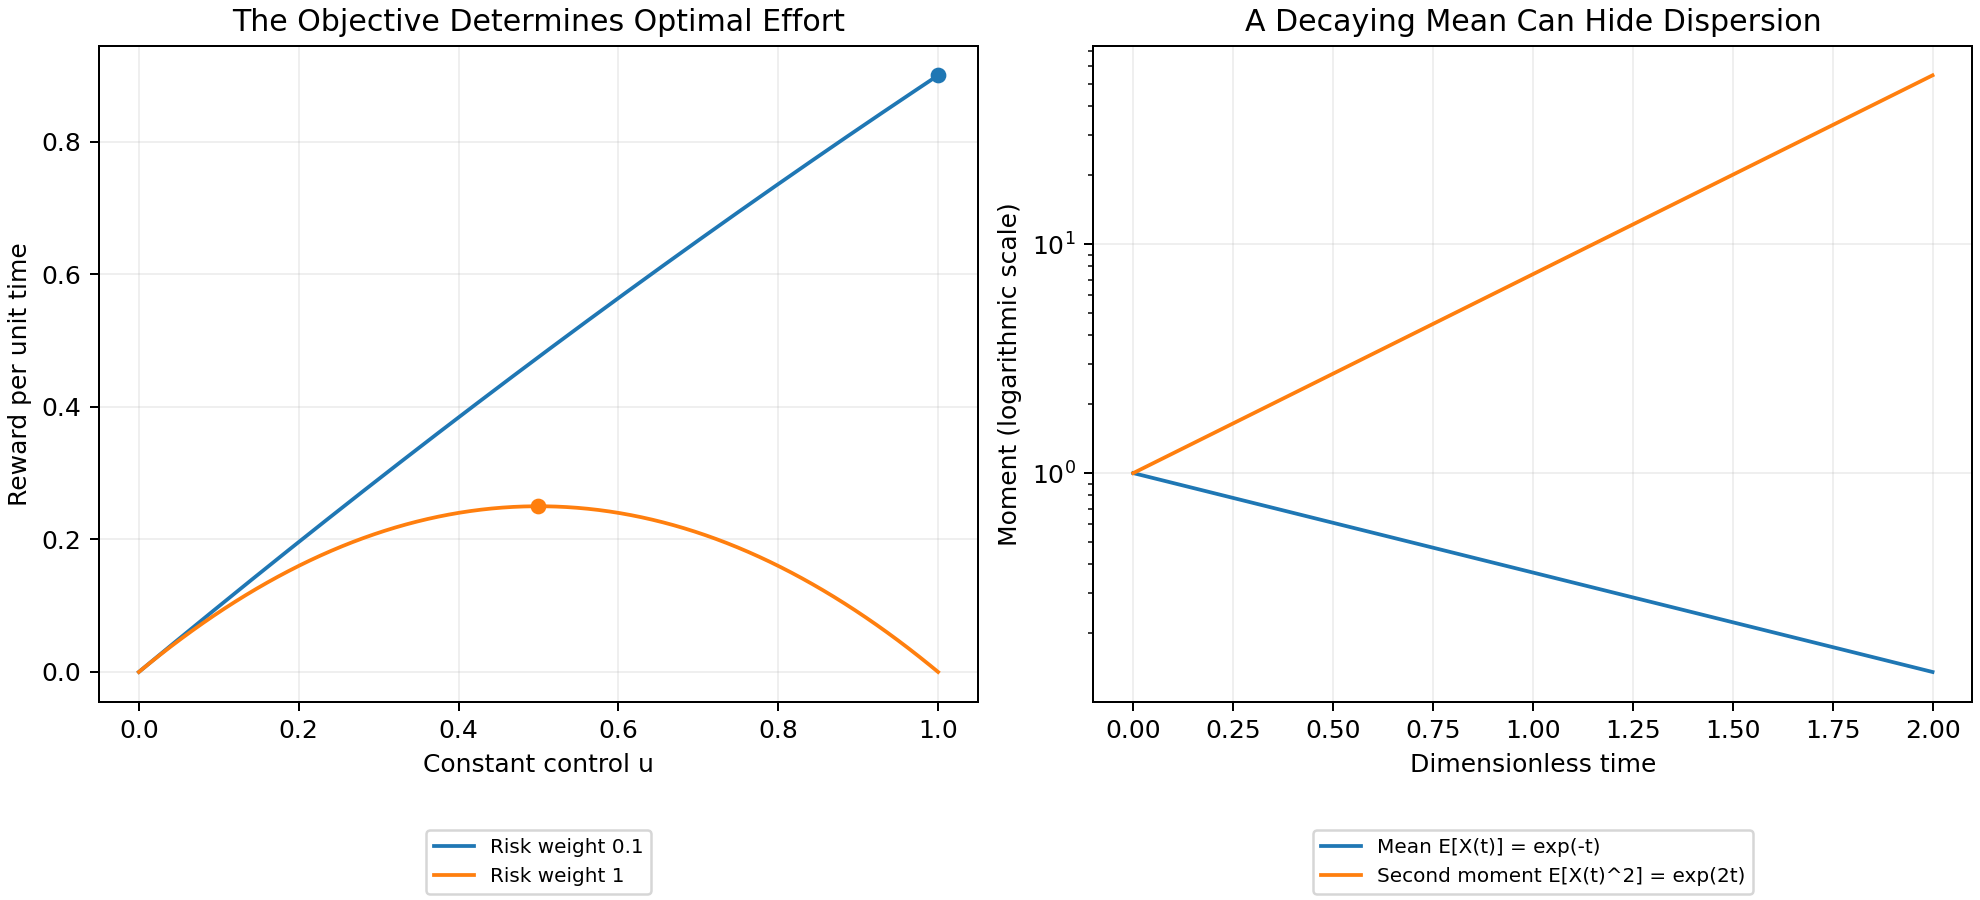
\includegraphics[width=\linewidth]{../The_Geometry_of_Motion/figures/stochastic_effort_examples.png}
\caption{Noise Changes the Optimization Problem}
\end{figure}

The calculated curves compare the two scalar reward functions and the separate multiplicative-noise example with a decaying mean but growing second moment. They are illustrative mathematical systems, not fitted human performance curves.

Fitts's original experiments relate movement duration to target amplitude and tolerance in particular motor tasks. A familiar fitted form is
\begin{equation}
T=a+b\log_2(2D/W),
\end{equation}
with $D$ the movement amplitude and $W$ the target width. It is not a theorem that increasing effort worsens every shot. Applying such a relationship to golf requires defining the task, tolerances, outcome distribution, and range over which a fitted model is supported. A fixed-position target acquisition task and high-speed moving club-ball contact have different terminal requirements.

\section{Risk, Reachability, and Contact Events}

For a task error $Z$ with mean $\mu$, covariance $\Sigma_Z$, and fixed positive-semidefinite weight $W$, the exact quadratic-loss identity is
\begin{equation}
\mathbb E[Z^\top WZ]=\mu^\top W\mu+\operatorname{tr}(W\Sigma_Z).
\end{equation}
Minimizing variance alone can retain a systematic miss. Include mean error and the appropriate performance reward. If the loss is strongly nonlinear or tail events matter, first and second moments may not determine expected loss or failure probability.

A smooth value function for a fixed-terminal-time Itô control problem formally satisfies the stochastic dynamic-programming equation
\begin{equation}
0=V_t+\min_u\left\{L+V_x f+
\tfrac12\operatorname{tr}(GG^\top V_{xx})\right\},
\end{equation}
with its terminal condition and admissibility assumptions. The diffusion term arises from Itô's formula. Event termination, partial observation, and nonsmooth values require additional treatment. Stochastic optimal control is not obtained by merely adding an unspecified uncertainty penalty to a deterministic Pontryagin Hamiltonian; the stochastic maximum principle is a separate framework with its own hypotheses.

One risk-sensitive criterion is $J_\theta=\theta^{-1}\log\mathbb E[e^{\theta C}]$, when the exponential moment exists. If the moment-generating function is finite around zero, the small-$\theta$ expansion is $\mathbb E[C]+\tfrac{\theta}{2}\operatorname{Var}(C)+O(\theta^2)$. Positive $\theta$ penalizes dispersion of cost locally in this expansion. It is not an arbitrary entropy term or a guarantee that every realization succeeds.

Define stochastic reachability explicitly, for example as a probability of reaching an acceptable impact set before leaving an admissible region. A Gaussian disturbance has unbounded support; a certificate proved only for bounded disturbances does not automatically cover all Gaussian realizations. A chance constraint, a mean-square bound, and a robust invariant tube quantify different properties. Deterministic Lie-algebra rank does not assign a probability to successful contact.

If contact occurs at a random first-hit time $\tau$, evaluate the appropriate output at $X_{\tau^-}$ and through the declared reset, rather than blindly using a fixed-time covariance. The guard equation is zero at contact by construction; that does not make clubface orientation or launch direction error zero. Event-time sensitivity and grazing contact can invalidate a simple fixed-time linearization.

\section{Phase, Measurement, and a Testable Swing Model}

For a smooth phase function $s=\phi(X)$ under closed-loop Itô dynamics, the chain rule becomes
\begin{equation}
ds=\left[\nabla\phi^\top f+
\tfrac12\operatorname{tr}(GG^\top D^2\phi)\right]dt
+\nabla\phi^\top G\,dW .
\end{equation}
The second-derivative term changes phase drift, and nonzero diffusion along the phase generally prevents strictly monotone sample paths. Positive expected progress does not restore the deterministic monotonicity assumption of Chapter 8. A filtered physical progress variable, event-based phase estimator, or colored-noise model must state how it handles this distinction.

Build a golf analysis in stages: identify the mechanical and observation models; estimate force-noise statistics at a stated bandwidth; propagate initial-state and process uncertainty under the actual feedback and limits; then evaluate first-contact outcomes. Include estimation errors and delays rather than granting the controller exact state information. Linear-quadratic-Gaussian separation results do not automatically apply to control-dependent diffusion, nonlinear contacts, or constrained actuators.

Validate the numerical model by checking time-step convergence with correctly scaled increments, comparing moment calculations with independent simulations where applicable, and reporting uncertainty in estimated failure rates. Validate its golf interpretation using held-out participants or swings, conditions, and perturbations appropriate to the claim. A model predicting lower dispersion at a chosen effort does not establish the athlete's internal objective or a universal coaching rule.

\section{Primary Reading}

\href{https://wolpertlab.neuroscience.columbia.edu/sites/default/files/content/papers/JonHamWol02.pdf}{Jones, Hamilton, and Wolpert (2002)} reports the isometric force study.
\href{https://wolpertlab.neuroscience.columbia.edu/sites/default/files/content/papers/HarWol98.pdf}{Harris and Wolpert (1998)} presents the minimum-variance model.
\href{https://pubmed.ncbi.nlm.nih.gov/4020415/}{Flash and Hogan (1985)} develops the reaching model.
\href{https://doi.org/10.1037/h0055392}{Fitts (1954)} reports the original amplitude-and-tolerance experiments.
\href{https://users.aalto.fi/~ssarkka/pub/sde_book.pdf}{Särkkä and Solin (2019)} provides background on stochastic calculus, moment equations, and numerical simulation.

\begin{samepage}
\section{Worked Checks and Exercises}

\begin{enumerate}[itemsep=0.25em,parsep=0pt]
\item Derive the variance produced by correct and incorrect noise increments under time-step refinement.
\item Calculate the first two moments of geometric Brownian motion and distinguish mean from mean-square stability.
\item Recover the multiplicative term in the linear covariance equation using Itô's product rule.
\item Verify the two equal-displacement controls with different peak commands and terminal variances.
\item Derive the minimum-jerk quintic and its cost; explain why it does not determine torque.
\item Solve the bounded scalar mean-variance optimization for both stated risk weights.
\item Separate bias and variance in an impact-error objective and identify the information moments omit.
\item State the difference between a bounded-disturbance funnel and a probabilistic first-contact success claim.
\end{enumerate}
\end{samepage}

\end{document}
